\section{Background and Proposed PENN Architecture}\label{sec:arch}

Before explaining the high level organization of PENN
architecture, we define the five specialization principles 
we employed to consider this style of architecture.
Our primary insight on coming to the architectural substrate
is based on well-understood mechanisms of specialization used in DSAs.
We first explain the assumptions we make for neural network workloads based on
our preliminary analysis.

\paragraph{Workload Assumptions}
1. Neural network workloads have significant parallelism, 
either at the data or thread level. 2. They perform some problem specific complex 
computational work and not just data-structure traversals. 3. They have coarse grain units of work. 
4. They have regular memory access patterns.

\subsection{Specialization Principles}

Broadly, we see these principles as a counterpart to the insights from Hameed et
al.~\cite{gpp_innef}, in that they describe the sources of inefficiency in a
general purpose processor, whereas our findings are oriented around
elucidating the sources of potential efficiency gain from specialization.  

\paragraph{Concurrency Specialization}
The concurrency of a workload is the degree to which its operations can be performed
in parallel. This concurrency can be derived from data or thread level parallelism
found in the workloads. 
Examples of specialization strategies
include employing many independent processing elements with their own controllers,
or using a wide vector model with a single controller.
We chose the former one as baseline architecture having many processing elements
with a low-power controller.

\paragraph{Computation Specialization}  
Computations are individual units of work in an algorithm executed by
functional units (FUs).
Specializing \emph{computation} means creating problem-specific FUs.  
For instance, a \texttt{sin} FU would much more efficiently compute the sine function than
iterative methods on a general purpose processor.
Specializing computation improves performance and energy by
reducing the total work.
Most of the neural network applications employ some commonality
in FU types.

\paragraph{Communication Specialization} 
Communication is the means of transmission of transient
values between the storage and functional units.  Specialized
communication is simply the instantiation of communication channels, and
potentially buffering, between FUs to ultimately facilitate a faster
operand throughput to the FUs.  This reduces power by lessening access
to intermediate storage, and potentially area if the alternative is a general
communication network.  

\paragraph{Data Reuse Specialization} 
Data reuse is an algorithmic property where intermediate
computed values are consumed multiple times.  
The specialization of data reuse means using
custom storage structures or reuse buffers for these temporaries.
Specializing reuse benefits performance and power by avoiding 
the more expensive access to a larger global memory or register files.

\paragraph{Coordination Specialization} 
Hardware coordination is the management of multiple hardware
units and their timing to perform  work.  Instruction
sequencing, control flow, interrupts handling and address generation are all
examples of coordination tasks.  
Specializing it usually involves the
creation of small finite state machines to perform each task.
A low-power in-order core or a micro-controller could be used for this coordination specialization.

\subsection{PENN Architecture}

\begin{figure}
  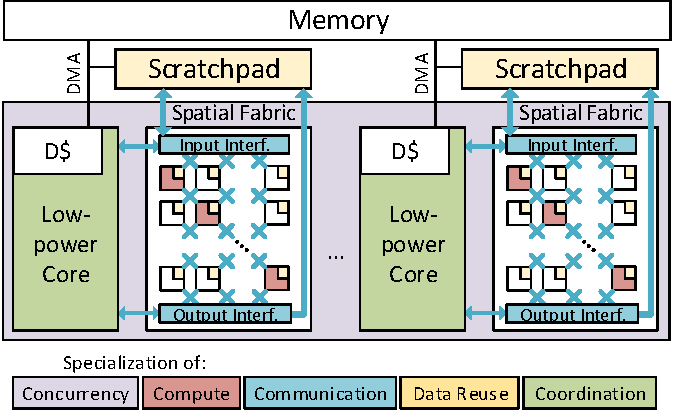
\includegraphics[width=\linewidth]{figs/fabric_5p.pdf}
  \vspace{-0.1in}
  \caption{Programmable Engine for Neural Networks (PENN) Architecture \textnormal{\small }  }
  \label{fig:penn-fabric}
\end{figure}

Figure~\ref{fig:penn-fabric} gives a high level overview of the PENN architecture 
we have proposed. 
The requirement to exploit high concurrency in workloads pushes the design towards simplicity, 
and the requirement of programmability implies the use of some sort of programmable core.
The natural way to fill these combined requirements is to use an array of tiny
low-power cores which communicate through memory.
These low power cores have caches, general purpose programmable and
are basic building blocks of PENN. The low-power core along with
other specialization units (explained below) form one unit of PENN fabric and
multiple such units are used to specialize \emph{Concurrency}.
Using many units, as opposed to a wide-vector model, has a flexibility advantage.  When
memory locality is not possible, parallelism can still be achieved through
multiple execution threads.  The remainder of the design is to straight-forwardly
apply the remaining specialization principles.

Achieving \emph{communication} specialization of intermediate values requires
an efficient distribution mechanism for operands, which avoids expensive
intermediate storage like multi-ported register files.  Arguably, the best
known way to do this is to use an explicit routing network, which is exposed to
the ISA to eliminate the hardware burden of dynamic routing.  This property is
what defines spatial architectures and therefore we add a spatial
architecture as our first mechanism. The spatial architecture 
can be a Coarse Grain Reconfigurable Fabric (CGRA) which has an
intermix of FUs connected spatially through an interconnected network. 
This serves two additional purposes.
First, it is an appropriate place to instantiate custom functional units, i.e.
\emph{computation} specialization.  Second, it accommodates \emph{reuse} of
constant values associated with specific computations.  In principle, this
spatial architecture can be either fine-grain reconfigurable (FPGA) or more
coarse grain reconfigurable.

To achieve \emph{communication} specialization with the global memory, a natural
solution is to add a DMA engine and configurable scratchpad, with a vector
interface to the spatial architecture.  The scratchpad, configured as a DMA
buffer, enables the efficient streaming of memory by decoupling memory access from the
spatial architecture.  When configured differently, the scratchpad can act as a
\emph{reuse} buffer.  In either context, a single-ported scratchpad is
enough, as access patterns are usually simple and known ahead of time.

Finally, we require an efficient mechanism for \emph{coordinating} the above
hardware units (e.g. configuring the spatial architecture or
synchronizing DMA with the computation).  Again, here we propose relying on the
simple core, as this brings a huge programmability and generality benefit.
Furthermore, the cost is low; if the core is low-power enough, and the spatial 
architecture is large enough, the overheads of coordination can be kept low.

To summarize, each unit of our proposed architecture contains a Low-power core,
a Spatial architecture, Scratchpad and DMA.
This architecture satisfies the programmable accelerator requirements:
general-purpose programmability, efficiency through the application of
specialization principles, and simple parameterizability.


\paragraph{PENN in Practice}

Preparing the PENN for use occurs in two phases: 
1. \emph{design synthesis} -- the selection of hardware parameters to suit the chosen workload
domain; and 2. \emph{programming} -- the generation of the program and spatial
datapath configuration to carry out the algorithm.

For our project, though many optimization strategies are possible, 
we  want to consider the 
primary constraint of this programmable architecture to be performance -- i.e. there
exists some throughput target that must be met, and power and area should be
minimized, while still retaining some degree of generality and programmability. 
We want to explore micro-architectural design decisions needed to make this
design synthesis step easier and efficient for many workload kernels.

Programming PENN has two major components: creation of the coordination
code for the low power core and generation of the configuration data/stream for the
spatial datapath to match available resources.  
In practice using standard languages with
\texttt{\#pragma} annotations, or even languages like OpenCL would likely be more
effective.  
Though we do not aim to implement a full-working compiler in this project,
we want to develop an API for PENN programming and hand-generate assembly instructions
along with configuration stream to configure PENN.
Figure~\ref{fig:ex-prog} shows an example annotated code for computing 
a neural network layer, along with a provisioned (already synthesized) PENN.  
The figure also shows the compilation steps to map each portion of the code to the 
architecture.  At a high level, the compiler will use annotations to identify
arrays for use in the SRAM, and how should they be used (either as a stream buffer or scratchpad). 
In the example, the weights can be loaded into the scratchpad, and reused across
invocations.
 
Subsequently, the compiler will unroll and create a large-enough datapath to
match the resources present in the spatial fabric, which could be spatially
scheduled using scheduling techniques. Communication
instructions would be inserted into the coordination code, as well as
instructions to control the DMA access for streaming inputs.  Finally, the
coordination loop would be modulo scheduled to effectively pipeline the spatial
architecture.

\begin{figure}
  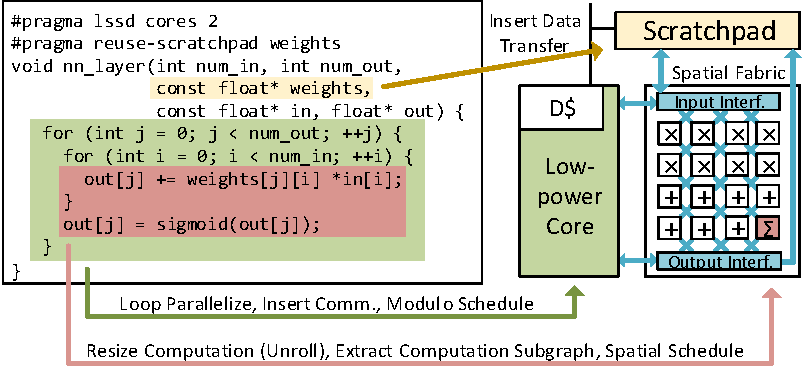
\includegraphics[width=\linewidth]{figs/example_prog.pdf}
  \vspace{-0.1in}
  \caption{Example Program \& Compiler Passes \newline
  \textnormal{\small (Arrows labeled with required compilation passes.)} 
}
  \label{fig:ex-prog}
\end{figure}

